\section{Stabilizing Deep Learning: Activations, Normalization, and Regularization}
\markright{2.7.\ Stabilizing Deep Learning}
\thispagestyle{plain}

The previous sections explained why deep networks are difficult to optimize.
Gradients can vanish or explode, signal scale can drift across depth, and highly expressive models can become statistically brittle even when optimization succeeds.
Modern deep learning became practical only when the field learned how to control all three of these issues at once.

\medskip

This section organizes that story into three subthemes:
\begin{itemize}
    \item \textbf{activation choice and gradient flow,}
    \item \textbf{normalization and scale control,}
    \item \textbf{regularization and generalization support.}
\end{itemize}

\medskip

These are not isolated tricks.
They are complementary ways of making deep learning both trainable and useful.
Activation functions shape the local derivatives through which signals move.
Normalization keeps internal representations in controlled numerical coordinates.
Regularization biases training toward solutions that are less brittle and more likely to generalize.

\subsection*{Activation choice and gradient flow}

A hidden layer has the form
\[
h^{(\ell)}=\phi\bigl(z^{(\ell)}\bigr),
\qquad
z^{(\ell)}=W^{(\ell)}h^{(\ell-1)}+b^{(\ell)}.
\]
During backpropagation the local gradient is multiplied by
\[
\phi'\bigl(z^{(\ell)}\bigr).
\]
So activation choice matters not only for expressivity, but also for whether gradients remain informative.

\medskip

This leads to a useful design principle.
One prefers activations whose derivative behavior supports learning in the regimes actually visited by the network.
If the derivative is almost always tiny, then gradient flow weakens.
If the activation truncates too aggressively, useful signal can be lost.
If the activation preserves a healthy range of derivatives, optimization becomes easier.

\begin{figure}[tbp]
\centering
\begin{minipage}[t]{0.48\textwidth}
\centering
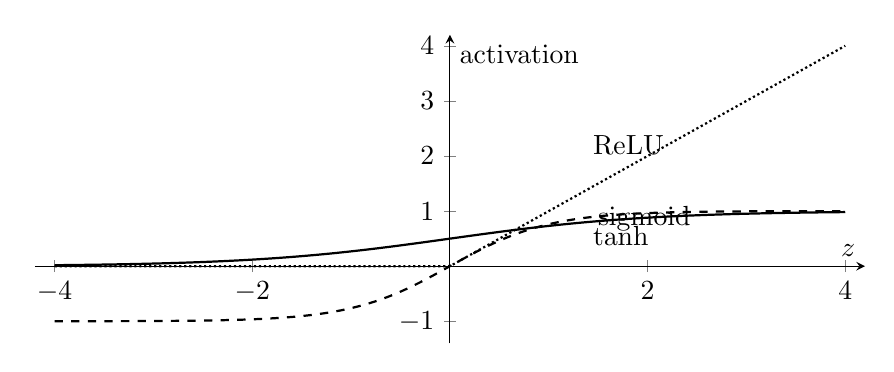
\begin{tikzpicture}
\begin{axis}[
    width=\textwidth,
    height=5.5cm,
    axis lines=middle,
    xmin=-4.2,xmax=4.2,
    ymin=-1.4,ymax=4.2,
    xlabel={$z$},
    ylabel={activation},
    xtick={-4,-2,0,2,4},
    ytick={-1,0,1,2,3,4},
    domain=-4:4,
    samples=250,
    clip=false,
]
\addplot[thick] {1/(1+exp(-x))};
\addplot[thick,dashed] {tanh(x)};
\addplot[thick,densely dotted] {x < 0 ? 0 : x};
\node[anchor=west] at (axis cs:1.4,0.86) {sigmoid};
\node[anchor=west] at (axis cs:1.35,0.55) {$\tanh$};
\node[anchor=west] at (axis cs:1.35,2.2) {ReLU};
\end{axis}
\end{tikzpicture}
\subcaption{Representative activation curves.}
\end{minipage}
\hfill
\begin{minipage}[t]{0.48\textwidth}
\centering
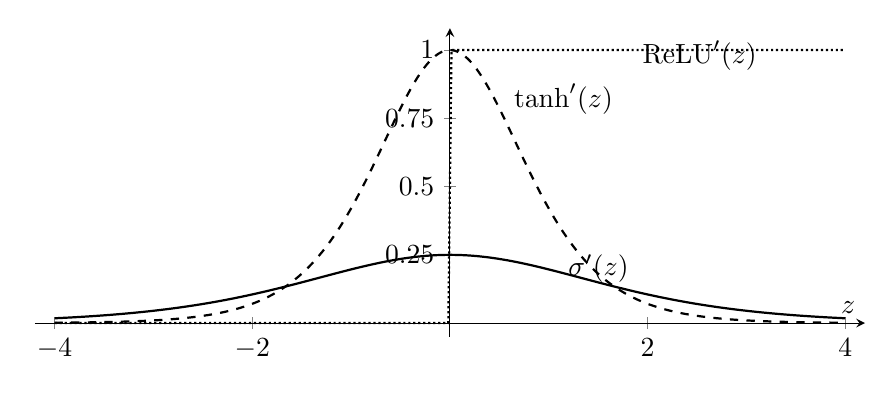
\begin{tikzpicture}
\begin{axis}[
    width=\textwidth,
    height=5.5cm,
    axis lines=middle,
    xmin=-4.2,xmax=4.2,
    ymin=-0.05,ymax=1.08,
    xlabel={$z$},
    xtick={-4,-2,0,2,4},
    ytick={0,0.25,0.5,0.75,1},
    domain=-4:4,
    samples=250,
    clip=false,
]
\addplot[thick] {(1/(1+exp(-x)))*(1-1/(1+exp(-x)))};
\addplot[thick,dashed] {1-(tanh(x))^2};
\addplot[thick,densely dotted] {x < 0 ? 0 : 1};
\node[anchor=west] at (axis cs:1.1,0.2) {$\sigma'(z)$};
\node[anchor=west] at (axis cs:0.55,0.82) {$\tanh'(z)$};
\node[anchor=west] at (axis cs:1.85,0.98) {$\mathrm{ReLU}'(z)$};
\end{axis}
\end{tikzpicture}
\subcaption{Derivative behavior drives gradient flow.}
\end{minipage}
\caption{Activation choice affects trainability because the derivative profile determines how strongly backpropagated information is attenuated or preserved. Sigmoid and $\tanh$ can saturate in their tails, while ReLU preserves derivative $1$ on its active side but becomes inactive on its negative side.}
\end{figure}

\paragraph{Sigmoid and \texorpdfstring{$\tanh$}{tanh}.}
These are smooth and bounded activations.
Their historical importance is enormous, but they saturate for large $|z|$.
In those regions the derivative is small, so repeated multiplication through depth weakens gradients.
The centering of $\tanh$ around zero often makes it easier to optimize than sigmoid, but the saturation problem remains.

\paragraph{ReLU and its descendants.}
The rectified linear unit
\[
\mathrm{ReLU}(z)=\max(0,z)
\]
avoids saturation on its positive side.
When a unit is active, the derivative is exactly $1$.
This helped make much deeper models trainable in practice.
Its cost is asymmetry: inactive units have output and derivative both equal to zero.
Leaky variants and smoother functions such as GELU can be viewed as attempts to preserve the trainability advantages of ReLU while softening its hard cutoff.

\medskip

The broad lesson is that activation functions should be judged not only by the functions they can represent, but also by the gradient environments they create.

\subsection*{Normalization and scale control}

Activation choice addresses one part of the signal-propagation problem.
Normalization addresses another.
Its core purpose is to keep internal representations in a numerically manageable range while learning is changing the network underneath them.

\begin{definition}[Batch normalization]
Let $z_{1},\dots,z_{m}$ denote the scalar values of one feature across a minibatch of size $m$.
Define the batch mean and variance by
\[
\mu_B=\frac{1}{m}\sum_{i=1}^m z_i,
\qquad
\sigma_B^2=\frac{1}{m}\sum_{i=1}^m (z_i-\mu_B)^2.
\]
Batch normalization forms the normalized coordinate
\[
\widehat z_i=\frac{z_i-\mu_B}{\sqrt{\sigma_B^2+\varepsilon}},
\]
and then applies a learned affine reparameterization
\[
y_i=\gamma \widehat z_i+\beta.
\]
Thus the feature is standardized across the examples of the minibatch before being rescaled and recentered by learned parameters.
\end{definition}

\begin{definition}[Layer normalization]
Let $z=(z_1,\dots,z_d)$ denote the feature vector for one example.
Define the within-example mean and variance by
\[
\mu_L=\frac{1}{d}\sum_{j=1}^d z_j,
\qquad
\sigma_L^2=\frac{1}{d}\sum_{j=1}^d (z_j-\mu_L)^2.
\]
Layer normalization forms
\[
\widehat z_j=\frac{z_j-\mu_L}{\sqrt{\sigma_L^2+\varepsilon}},
\qquad
y_j=\gamma_j \widehat z_j+\beta_j.
\]
Thus normalization is performed across features of a single example rather than across a minibatch.
\end{definition}

\medskip

These definitions look similar because the core mechanism is similar: convert a raw internal coordinate into a standardized one and then allow the network to relearn an appropriate scale and offset.
The practical difference is where the statistics are computed.
Batch normalization couples examples within a minibatch.
Layer normalization acts within one example and is therefore natural in sequence models and transformers.

\begin{proposition}[Normalization changes scale sensitivity and optimization geometry]
Consider an idealized normalization layer with $\varepsilon=0$.
Suppose a scalar pre-activation is multiplied by a positive constant $c>0$, so that $z_i'=c z_i$.
Then the normalized coordinate is unchanged:
\[
\frac{z_i'-\mu'}{\sigma'}
=
\frac{z_i-\mu}{\sigma},
\]
where $\mu',\sigma'$ are the mean and standard deviation computed from $z_1',\dots,z_m'$ in batch normalization or from the feature vector $z'$ in layer normalization.
Consequently, normalization removes sensitivity to raw positive rescaling along certain directions, so it changes the effective optimization geometry rather than merely changing output values.
\end{proposition}

\begin{proof}
If $z_i'=c z_i$, then the corresponding mean rescales as $\mu'=c\mu$.
Likewise the standard deviation rescales as $\sigma'=c\sigma$ because variance rescales by $c^2$.
Therefore
\[
\frac{z_i'-\mu'}{\sigma'}
=
\frac{c z_i-c\mu}{c\sigma}
=
\frac{z_i-\mu}{\sigma}.
\]
The same algebra holds whether the statistics are taken across a minibatch or across coordinates of one example.
Thus the normalized coordinate is invariant to positive rescaling of the underlying raw coordinate.
\end{proof}

This proposition explains why normalization is deeper than simple output rescaling.
It changes which parameter directions matter.
Scaling the incoming representation no longer affects the normalized coordinate in the same way it would in an unnormalized network.
So optimization takes place in a different geometry, with internal coordinates continually brought back toward a controlled range.

\begin{figure}[tbp]
\centering
\begin{tikzpicture}[>=Latex, node distance=0.95cm and 0.7cm]
\tikzset{box/.style={draw, fill=gray!10, rounded corners, minimum width=3.0cm, minimum height=1.45cm, align=center, font=\small}}
\node[box] (raw) {raw activations\\different means\\different variances};
\node[box, right=of raw] (norm) {normalize\\center around $0$\\scale near $1$};
\node[box, right=of norm] (affine) {learned affine step\\$\gamma \widehat z+\beta$\\task-appropriate scale};

\draw[thick,->] (raw) -- (norm);
\draw[thick,->] (norm) -- (affine);

\node[font=\small, align=center] at ($(raw.south)+(0,-1.05)$) {drifting internal\\scale};
\node[font=\small, align=center] at ($(norm.south)+(0,-1.05)$) {standardized\\coordinates};
\node[font=\small, align=center] at ($(affine.south)+(0,-1.05)$) {useful but\\controlled scale};
\end{tikzpicture}
\caption{Normalization as scale control. The point is not to freeze all internal values forever, but to keep the optimization operating in standardized coordinates and then let the network relearn a useful affine scale.}
\end{figure}

\commonconfusion{Batch normalization is \emph{not} the same thing as regularization, even though it can have regularizing side effects. Its primary role is optimization stabilization and scale control: it changes the coordinates in which learning happens and often makes training less sensitive to initialization or learning-rate choice. The minibatch noise it introduces may also regularize, but that is not the whole story and not the best first interpretation.}

\paragraph{Batch norm versus layer norm.}
The most important conceptual distinction is simple.
Batch normalization standardizes each feature across examples in a minibatch.
Layer normalization standardizes the full feature vector within one example.
So batch norm ties examples together during training, while layer norm does not.
That is why batch norm is often natural in convolutional settings with large minibatches, whereas layer norm fits sequence models and transformers where batch statistics are less central.

\subsection*{Regularization and generalization support}

Once optimization is stable enough to train a deep model, a second question emerges.
Why should the learned solution generalize rather than merely memorize?
Regularization methods address that question.
They do not primarily keep gradients numerically alive.
Instead, they bias the learning dynamics or the objective toward solutions that are less brittle.

\begin{remark}[Optimization stabilization versus statistical regularization]
It is useful to distinguish two roles that are often blurred together.
Methods such as normalization mainly stabilize optimization by controlling signal scale and changing the effective parameter geometry.
Methods such as dropout, weight decay, early stopping, and data augmentation mainly support generalization by discouraging fragile or overly specialized solutions.
In practice the boundary is not absolute: one method can have both optimization and regularizing effects.
But pedagogically the distinction is essential.
\end{remark}

\paragraph{Dropout.}
During training, dropout multiplies an activation vector $h$ by a random mask $m$ with entries in $\{0,1\}$.
In the common inverted-dropout convention,
\[
\widetilde h = \frac{m\odot h}{p},
\]
where $p$ is the keep probability.
Then each coordinate satisfies
\[
\mathbb E[\widetilde h_j]=h_j,
\]
so the expected activation scale is preserved even though random pathways are temporarily removed.
This encourages the network not to depend too strongly on any one co-adapted configuration of units.

\begin{figure}[tbp]
\centering
\begin{tikzpicture}[>=Latex, node distance=0.55cm and 0.55cm]
\tikzset{unit/.style={circle, draw, minimum size=0.45cm, inner sep=0pt}}
\foreach \y in {1,2,3,4} {
    \node[unit] (a\y) at (0,-0.8*\y) {};
    \node[unit] (b\y) at (2,-0.8*\y) {};
    \node[unit] (c\y) at (4,-0.8*\y) {};
}
\foreach \i in {1,2,3,4} {
    \foreach \j in {1,2,3,4} {
        \draw[gray!65] (a\i) -- (b\j);
        \draw[gray!65] (b\i) -- (c\j);
    }
}
\draw[line width=1.2pt, red] ($(b2)+(-0.23,0.23)$) -- ($(b2)+(0.23,-0.23)$);
\draw[line width=1.2pt, red] ($(b2)+(-0.23,-0.23)$) -- ($(b2)+(0.23,0.23)$);
\draw[line width=1.2pt, red] ($(b4)+(-0.23,0.23)$) -- ($(b4)+(0.23,-0.23)$);
\draw[line width=1.2pt, red] ($(b4)+(-0.23,-0.23)$) -- ($(b4)+(0.23,0.23)$);
\node[font=\small] at (0,0) {input};
\node[font=\small] at (2,0) {hidden};
\node[font=\small] at (4,0) {next layer};
\node[font=\small, align=center] at (2,-4.1) {dropout randomly removes\\some active pathways during training};
\end{tikzpicture}
\caption{A dropout mask schematic. Randomly suppressing units during training encourages the network to spread useful information across multiple pathways rather than relying on a single fragile configuration.}
\end{figure}

\paragraph{Weight decay, early stopping, and data augmentation.}
Weight decay penalizes large parameter norms and often biases learning toward less extreme solutions.
Early stopping halts training before the model fully fits sample-specific noise.
Data augmentation enlarges the effective training distribution by applying label-preserving transformations, thereby encouraging invariances that reflect the task structure.
These methods look different, but they share one aim: improve out-of-sample behavior by discouraging brittle fitting.

\medskip

Seen together, the conceptual division of labor is clear.
Activation choice helps gradients remain useful.
Normalization keeps internal scale under control.
Regularization guides optimization toward solutions that generalize better.
Modern deep learning relies on all three.

\subsection*{The central lesson}

The right summary is not simply that deep networks became better because they became larger.
They became practical because signal flow, scale control, and generalization support became manageable enough for large-scale optimization to work reliably.

\medskip

In that sense, modern deep learning is not only a story of expressive model classes.
It is equally a story of learning how to stabilize those classes during training.

\subsection*{Exercises}

\begin{exercise}
Compare sigmoid, $\tanh$, and ReLU from the perspective of derivative behavior.
Which of them saturate, in what regimes, and how does that affect gradient flow in a deep network?
Explain why an activation that is expressive enough in principle may still be a poor choice for optimization.
\end{exercise}

\begin{exercise}
Explain the difference between batch normalization and layer normalization.
Your answer should identify where the mean and variance are computed, why this changes the training behavior, and why layer normalization is often more natural in transformer-style architectures.
\end{exercise}

\begin{exercise}
Let dropout keep each coordinate independently with probability $p$, and use the inverted-dropout rule
\[
\widetilde h = \frac{m\odot h}{p}.
\]
Show informally that $\mathbb E[\widetilde h_j]=h_j$ for each coordinate.
Then explain why preserving the expectation does \emph{not} mean dropout leaves training unchanged.
What source of stochasticity remains?
\end{exercise}

\subsection*{Notes and references}

The purpose of this section is to separate three roles that are often mixed together in practice: activation design for gradient flow, normalization for internal scale control, and regularization for generalization support.
The exact theory behind normalization remains incomplete, but the scale-invariance proposition already captures an essential point: normalized networks are optimized in a different geometry from unnormalized ones.
That is why these methods should be seen not as isolated engineering tricks, but as structural answers to trainability and robustness in deep learning.
